\title{Chum Populations}

\documentclass[12pt,  one column]{article}
\usepackage{graphicx}

\begin{document}



\section*{Abstract}

\section*{Introduction}

\section*{Methods}

Dominance coding \cite{}

 - measure information loss
 
 
 


\subsection*{Effective population size}

\subsection*{Ascertainment Bias}

\section*{Results}

\subsection*{Linkage map}
Identification of paralogs

congruence of paralog across families (supplemental table)

Consensus linkage map

Table (Figure?)
placement of centromeres

table (supplemental)
paralogs
note the distribution of paralogs matches the  pattern found in other salmonids
syntenic relationships - per LG
Table (supplemental?)
Population genetics

Summarize population relationships
Figure of individual-based 4 PCAs

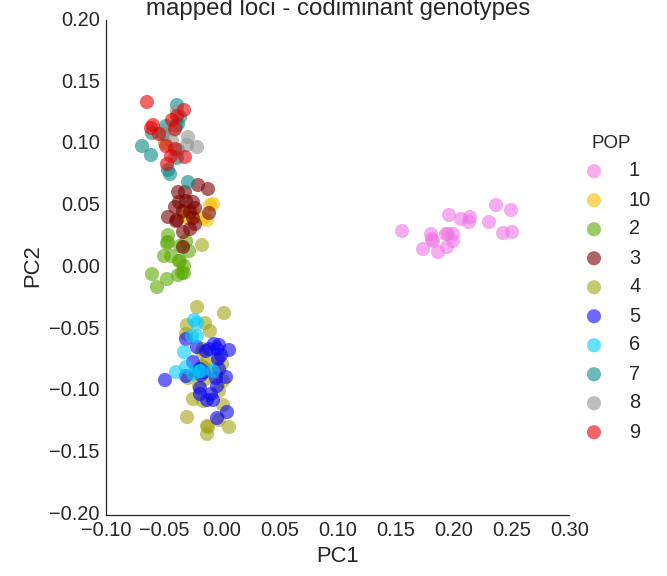
\includegraphics[scale=.3]{figures/PCA_codom.png}
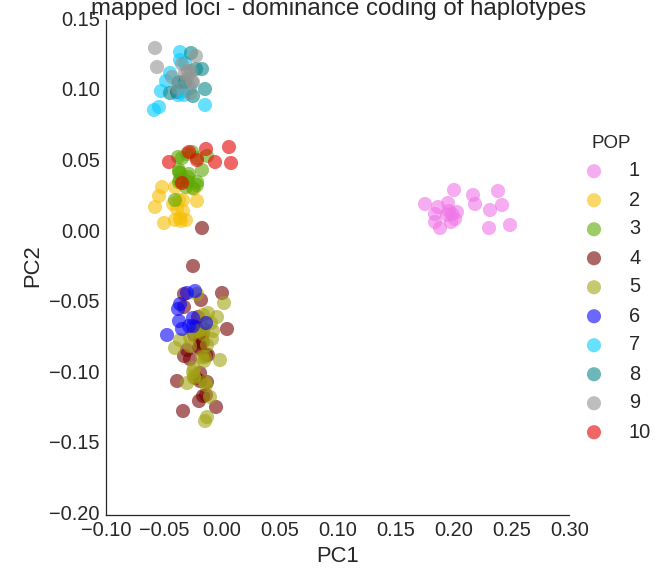
\includegraphics[scale=.3]{figures/PCA_dom.png}

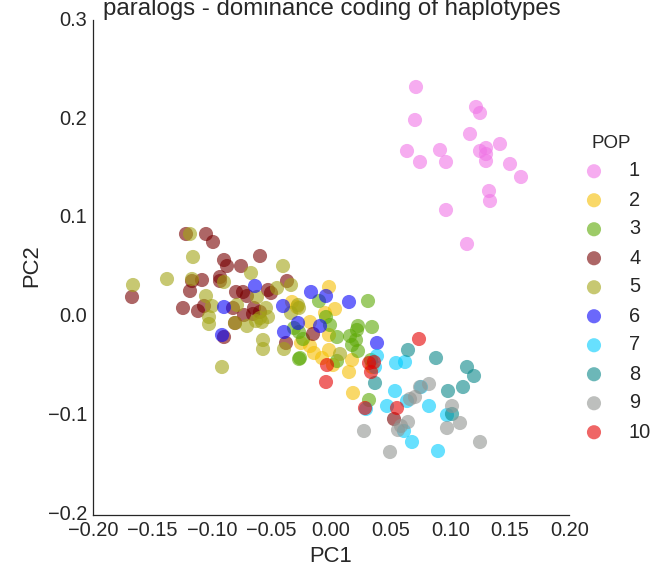
\includegraphics[scale=.3]{figures/PCA_dom_paralogs.png}
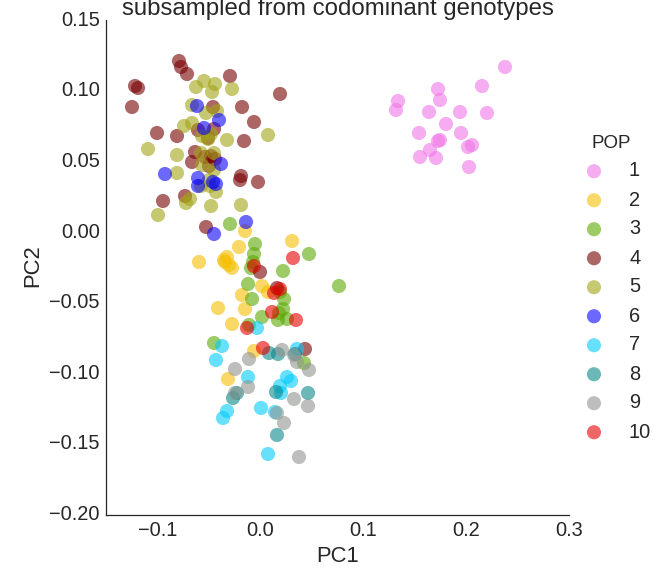
\includegraphics[scale=.3]{figures/PCA_codom_subsample.png}


measure information loss from dominance coding
discuss population vs individual based results
paralogs have similar neutral patterns of population structure.
can we demonstrate contained within paralogs by bootstrapping 
Genome scans (Outliers) - LG regions highlighted.

\subsection*{Effective population size}

\subsection*{Ascertainment Bias}
Demonstrate ascertainment effect when using only loci on linkage map - effect on allele frequencies.


\section*{Discussion}

\section*{Supplemental}

%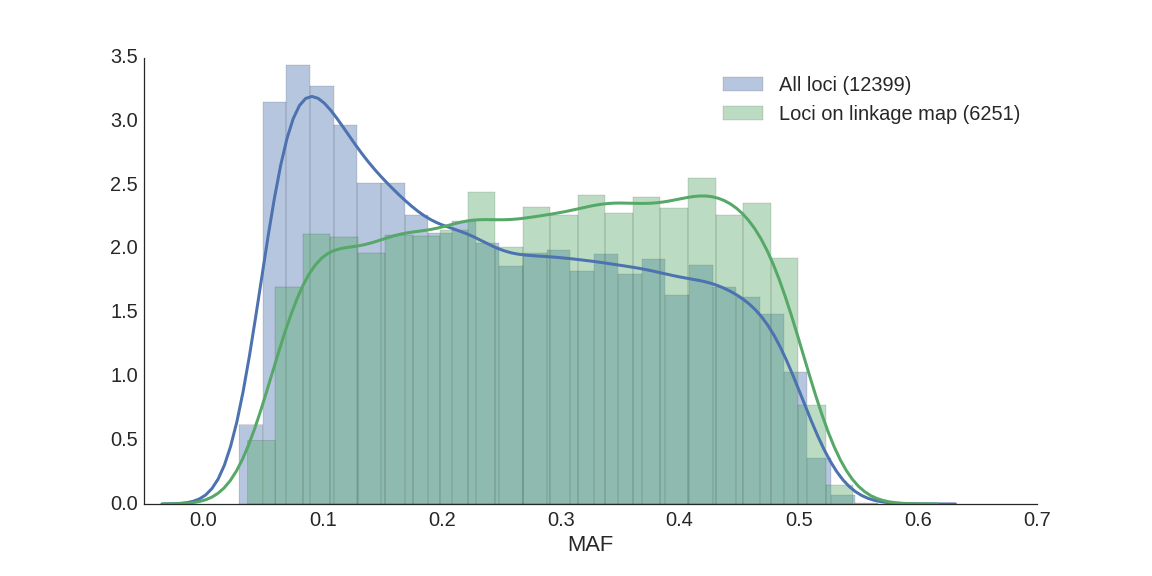
\includegraphics[scale=.4]{figures/supplemental/ascertainment.png}

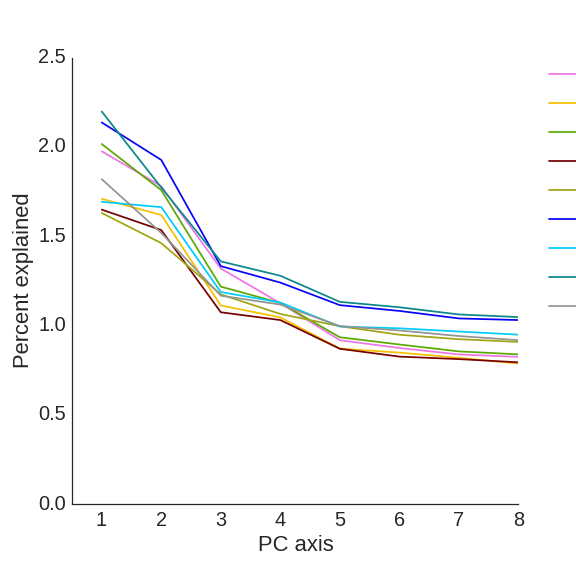
\includegraphics[scale=.4]{figures/supplemental/PCA_eigenvalues.png}

%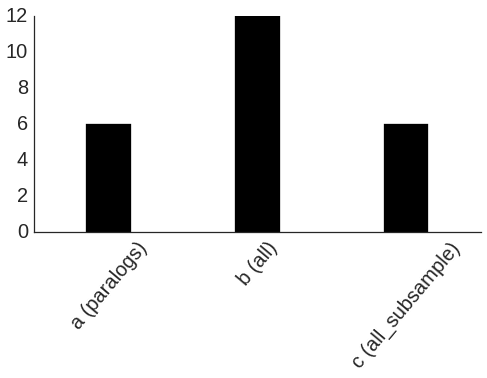
\includegraphics[scale=.4]{figures/supplemental/TW_stats.png}


%\begin{figure}
%\begin{center}
%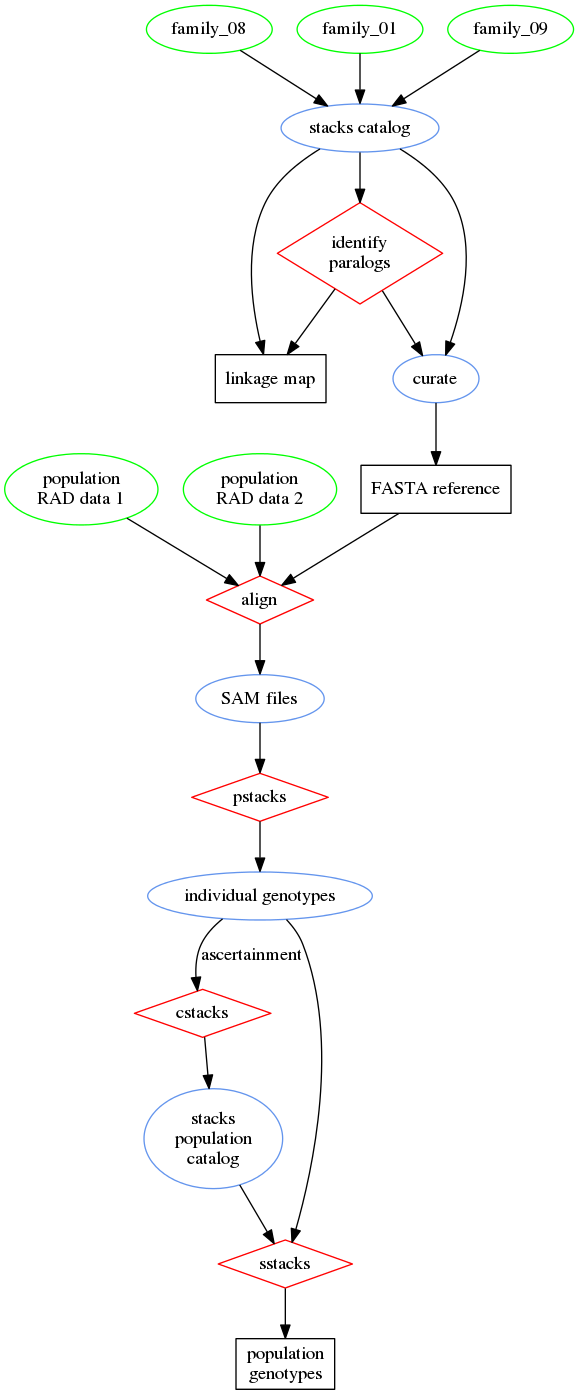
\includegraphics[scale=.3]{figures/supplemental/analysis_flowchart.png}
%\end{center}
%\end{figure}


\end{document}